\chapter{Metodologia}\label{chapter:metodologia}

% -----------------------------------------------------------------------------
% Capítulo 3.1 - Objetivos
% -----------------------------------------------------------------------------
\section{Objetivos}\label{section:objetivos}

Em resumo, o projeto propõe um protótipo de um nó IoT acionado pela Alexa. O protótipo comunicará com o serviço AWS IoT via tópicos MQTT - protocolo também utilizado na integração do AWS IoT com a Alexa. A \autoref{fig:project_diagram} mostra um diagrama em alto nível do projeto.

\begin{figure}[htbp]
    \centering
    \caption{Diagrama em alto nível do protótipo acionado pela Alexa e integrado ao serviço AWS IoT.}
    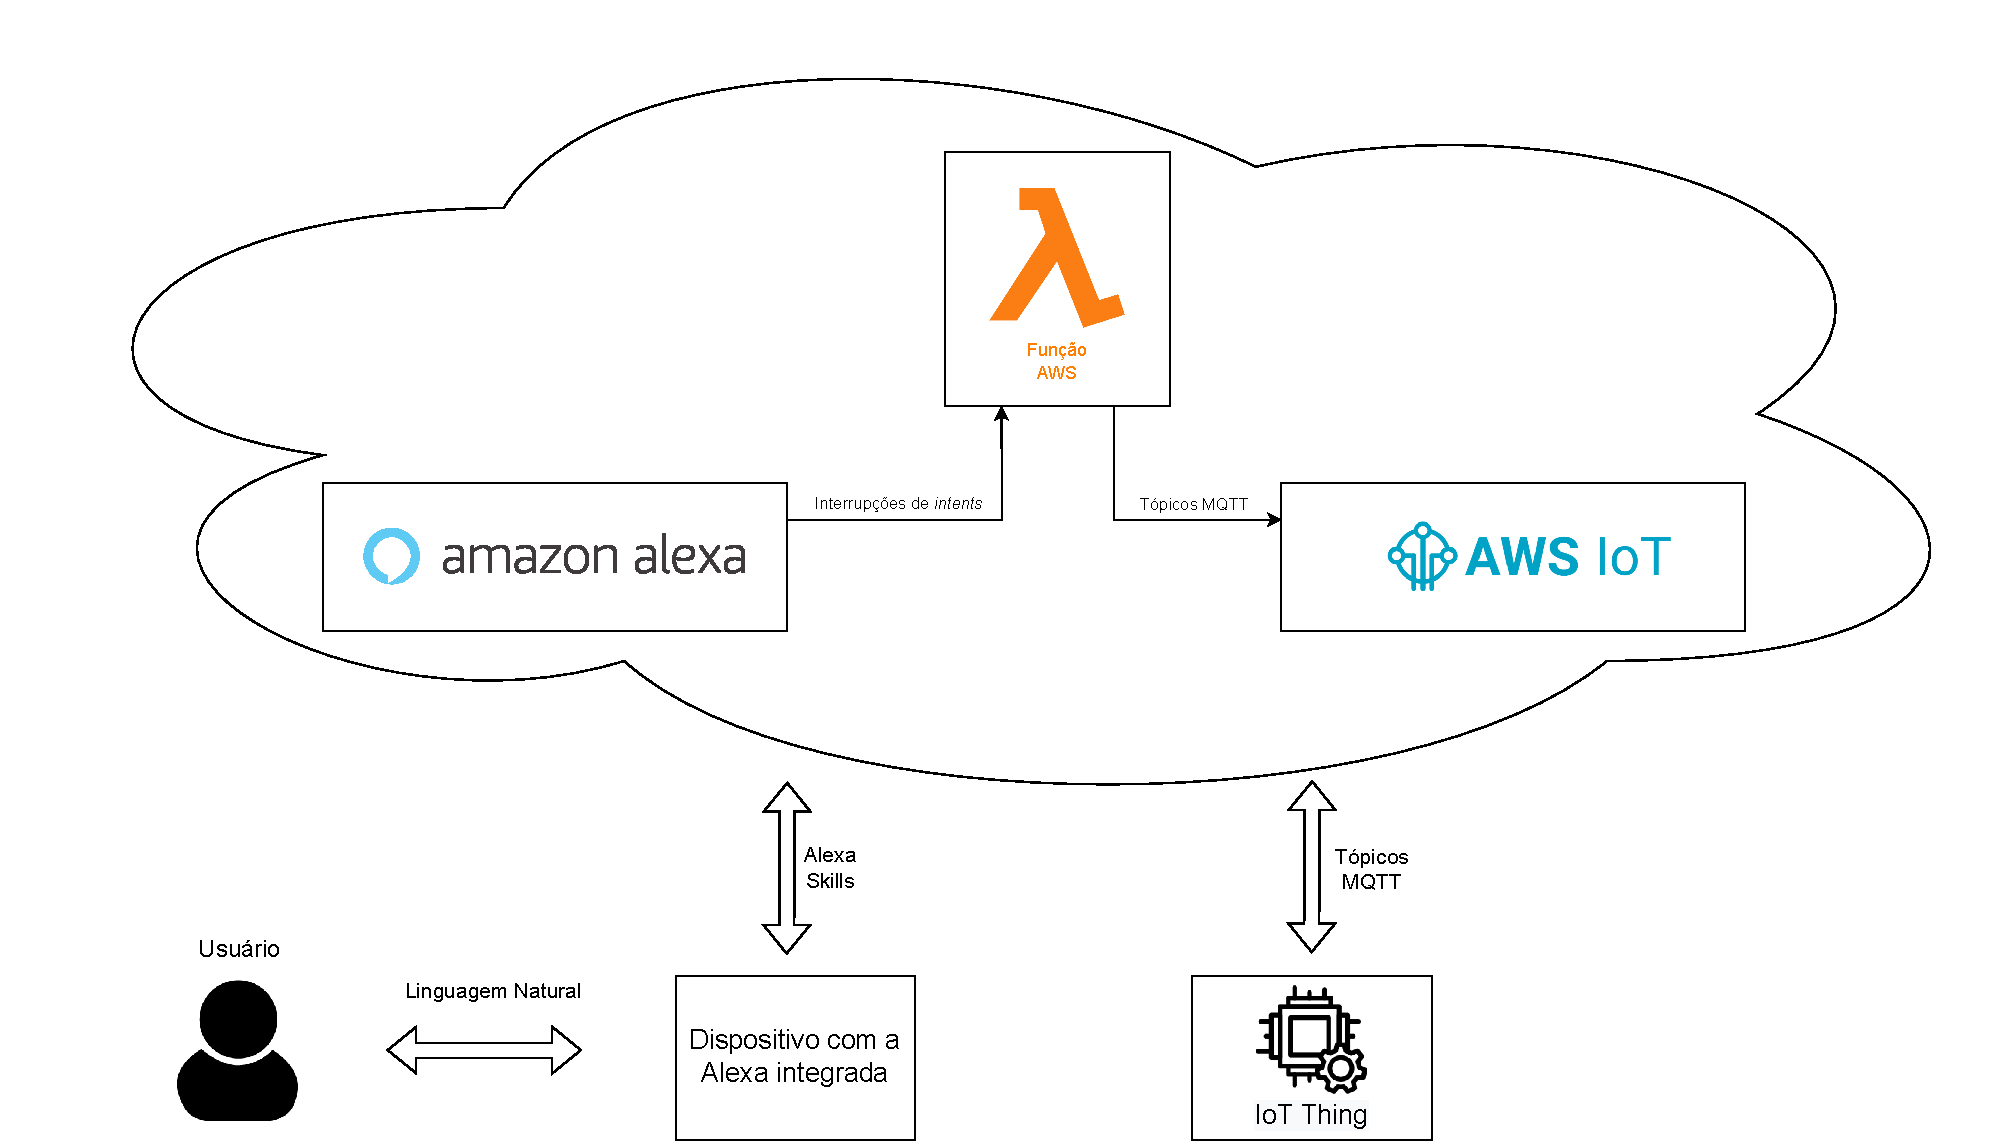
\includegraphics[scale=0.47]{Imagens/project_diagram.pdf}
    \legend{Fonte: Produzido pelo autor (2022).}
    \label{fig:project_diagram}
\end{figure}

Para esse dispositivo, tem-se os seguintes requisitos funcionais:

\begin{alineas}
    \item Suporte à rede Wifi IEEE 802.11 (2,4 GHz);
    \item Possibilidade de se comportar como um nó IoT;
    \item Suporte ao protocolo MQTT;
    \item Possibilidade de comunicação do usuário com o dispositivo em linguagem natural, a partir de microfones;
    \item Possibilidade de implementação de uma Alexa integrada;
    \item Possibilidade de acionamento da Alexa por voz ou toque;
    \item Microfones capazes de entender o usuário em ambientes ruidosos;
\end{alineas}

A seguir, tem-se os requisitos não-funcionais:

\begin{alineas}
    \item Ser um dispositivo qualificado pela AWS;
    \item Baixo custo de prototipagem;
    \item Versatilidade;
\end{alineas}

% -----------------------------------------------------------------------------
% Capítulo 3.2 - Projeto de Hardware
% -----------------------------------------------------------------------------
\section{Projeto de Hardware}

Uma vez escolhidos os requisitos funcionais e não-funcionais do projeto, inicia-se o projeto de hardware. Tomando o baixo custo de prototipagem como um importante requisito do projeto, optou-se pelo uso de sistemas embarcados no projeto. Computadores e notebooks pessoais, por exemplo, possuem um propósito geral e um alto valor agregado, enquanto um sistema embarcado realiza um conjunto de tarefas predefinidas e normalmente possuem um menor valor agregado \cite{ref:033}. Isso posto, inicia-se o estudo dos requisitos de um hardware a ser utilizado em aplicações IoT. Como um dos requisitos funcionais é a possibilidade de implementação de uma Alexa integrada, estuda-se os parâmetros mínimos recomendados pela AWS para um dispositivo com a Alexa integrada. Esses requisitos podem ser vistos na \autoref{table:reduced_hardware_footprint}.

\begin{table}[htbp]
    \centering
    \caption{Parâmetros mínimos recomendados pela AWS para o desenvolvimento de um dispositivo de IoT integrado à AVS.}
    \begin{tabular}{|c|c|}
        \hline
        \textbf{Processador}      & \begin{tabular}[c]{@{}c@{}}ARM M7 or equivalent\\ Arm M4 + AFE DSP\end{tabular} \\ \hline
        \textbf{RAM}              & \begin{tabular}[c]{@{}c@{}}MB for ARM M7\\ 500KB for M4 + AFE DSP\end{tabular}  \\ \hline
        \textbf{Target OS}        & FreeRTOS                                                                        \\ \hline
        \textbf{Conectividade}    & MQTT/Wi-Fi                                                                 \\ \hline
        \textbf{\# de Microfones} & 2+                                                                              \\ \hline
        \textbf{Alto-falante}     & Optimized for speech playback                                                   \\ \hline
    \end{tabular}
    \legend{Fonte: \cite{ref:034}}
    \label{table:reduced_hardware_footprint}
\end{table}

Para a prototipagem, alguns kits de desenvolvimento disponíveis no mercado foram estudados. As tabelas \autoref{table:development_kit_a} e \autoref{table:development_kit_b} mostram informações coletadas de cinco diferentes kits.

\begin{table}[htbp]
  \caption{kits de desenvolvimento recomendados pela Amazon para o desenvolvimento de aplicações IoT (A).}
  \begin{tblr}{@{}|X[c,valign=m,gray!30]|X[c,valign=m]|X[c,valign=m]|X[c,valign=m]|X[c,valign=m]|X[c,valign=m]|@{}}
      \hline
      \textbf{Número de produto}        & B-L475E-IOT01A2                                                           & CORE-V MCU DevKit                                                   & SLN-ALEXA-IOT                                  \\ \hline
      \textbf{Descrição}                & STM32L4 Discovery kit Nó IoT, low-power wireless, BLE, NFC, SubGHz, Wi-Fi & European RISC-V chip for IoT development kit                        & EdgeReady MCU Based Solution for Alexa for IOT \\ \hline
      \textbf{Processador}              & Arm® Cortex®-M4                                                           & CV32E40P processor core                                             & Arm® Cortex®-M7 Core                           \\ \hline
      \textbf{FreeRTOS}                 & Sim                                                                       & Não Disponível                                                      & Sim                                            \\ \hline
      \textbf{Conectividade}            & Inventek ISM43362 Wi-Fi Module                                            & Espressif AWS IoT ExpressLink Module for AWS IoT cloud interconnect & Bluetooth LE 4.2, 802.11 b/g/n Wi-Fi®          \\ \hline
      \textbf{Microfones}               & 2 digital omnidirectional microphones (MP34DT01)                          & Não Disponível                                                      & Digital MEMS microphones (x3)                  \\ \hline
      \textbf{Alto-falante}             & Não Disponível                                                            & Não Disponível                                                      & Não Disponível                                 \\ \hline
      \textbf{Preço nas Lojas Oficiais} & \$53,00                                                                   & Preços Individuais                                                  & \$171,35                                       \\ \hline
  \end{tblr}
  \legend{Fontes: \cite{ref:035}, \cite{ref:036}, \cite{ref:037}}
  \label{table:development_kit_a}
\end{table}

\begin{table}[htbp]
  \caption{kits de desenvolvimento recomendados pela Amazon para o desenvolvimento de aplicações IoT (B).}
  \begin{tblr}{@{}|X[c,valign=m,gray!30]|X[c,valign=m]|X[c,valign=m]|X[c,valign=m]|X[c,valign=m]|X[c,valign=m]|@{}}
      \hline
      \textbf{Número de produto}        & Home Hub 100 Dev Kit for Amazon AVS                                                                                                                                             & STEVAL-VOICE-UI                                                                                                                                                            \\ \hline
      \textbf{Descrição}                & A hardware and software development kit with multi-core connectivity designed to support AVS for AWS IoT Core connected devices                                                 & Qualified hardware reference design enabling easy and cost effective addition of the Alexa Voice Service (AVS) Integration for AWS IoT core to your smart embedded devices \\ \hline
      \textbf{Processador}              & Arm Cortex-M4F CPU                                                                                                                                                              & Dual Arm® Cortex®-A7 and Cortex®-M4 Cores                                                                                                                                  \\ \hline
      \textbf{FreeRTOS}                 & Sim                                                                                                                                                                             & Sim                                                                                                                                                                        \\ \hline
      \textbf{Conectividade}            & Integrated Bluetooth 5, Qualcomm® Bluetooth Mesh connectivity, low power Wi-Fi 802.11n in 2.4GHz/5GHz bands, and 802.15.4, with support for ZigBee3.0 and Thread via OpenThread & WIFI subsystem including Murata 1DX module used in bypass mode and ISSI IS25LP016D 2Mbytes NOR flash hosting WIFI low level software                                       \\ \hline
      \textbf{Microfones}               & Não Disponível                                                                                                                                                                  & 2 MP23DB01HP Microphone Mems                                                                                                                                               \\ \hline
      \textbf{Alto-falante}             & 1x                                                                                                                                                                              & 1x (8 ohm)                                                                                                                                                                 \\ \hline
      \textbf{Preço nas Lojas Oficiais} & £42.95                                                                                                                                                                          & \$248.75                                                                                                                                                                   \\ \hline
  \end{tblr}
  \legend{Fontes: \cite{ref:038}, \cite{ref:039}}
  \label{table:development_kit_b}
\end{table}

Assim como pode ser visto na \autoref{table:reduced_hardware_footprint}, A AWS recomenda o Sistema Operacional FreeRTOS, descartando o \textit{CORE-V MCU DevKit}. Ademais, definiu-se como requisito funcional a possibilidade de comunicação do usuário com o dispositivo através de linguagem natural, demandando no mínimo dois microfones e descartando o \textit{Home Hub 100 Dev Kit for Amazon AVS}.

Por fim, restando somente os dispositivos \textit{STEVAL-VOICE-UI}, \textit{B-L475E-IOT01A2} e \textit{SLN-ALEXA-IOT}, avaliou-se o preço nas lojas oficiais. Os preços, em Novembro de 2022, são respectivamente: \$248.75, \$51,94 e \$171,35. Essa discrepância de valores acontece devido à diferença nas especificações: o segundo dispositivo possui processador Arm® Cortex®-M4, enquanto o primeiro e o terceiro processadores Arm® Cortex®-M7 e Dual Arm® Cortex®-A7, respectivamente. Outrossim, os dispositivos \textit{STEVAL-VOICE-UI} e \textit{SLN-ALEXA-IOT} também contam com alto-falantes, já o \textit{B-L475E-IOT01A2} não. Vale lembrar que a possibilidade de comunicação do dispositivo com o usuário via alto-falante não é um requisito funcional do projeto.

Dessa forma, conclui-se que o kit \textit{B-L475E-IOT01A2} é o dispositivo, com menor custo, que mais se aproxima dos requisitos mínimos especificados pela AWS e atende os requisitos funcionais do projeto. O kit escolhido por ser visto na \autoref{fig:B-L475E-IOT01A2}.

\begin{figure}[htbp]
    \centering
    \caption{Kit de desenvolvimento escolhido para ser protótipo do projeto (\textit{B-L475E-IOT01A2}).}
    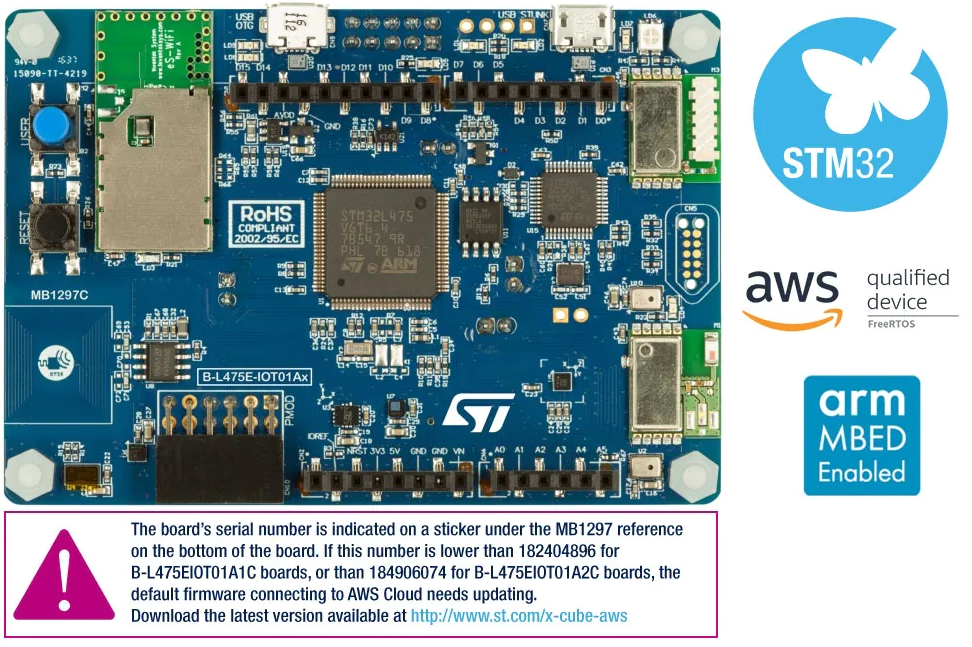
\includegraphics[scale=0.7]{Imagens/B-L475E-IOT01A2.png}
    \legend{Fonte: \cite{ref:035}.}
    \label{fig:B-L475E-IOT01A2}
\end{figure}

% -----------------------------------------------------------------------------
% Capítulo 3.3 - Criação de um nó IoT na rede AWS
% -----------------------------------------------------------------------------
\section{Criação de um nó IoT na rede AWS}\label{section:criacao_de_um_no_iot_na_rede_aws}

Um nó IoT é representado na AWS como uma coisa no serviço AWS IoT. Cada coisa, ou grupo de coisas, pertence a alguma região da AWS. Assim, o dispositivo de protótipo foi autenticado na região \textit{us-east-1} (N. Virginia) como \textit{B-L475E-IOT01A2}. O processo completo de criação, autenticação e autorização de uma coisa no AWS IoT se encontra na \autoref{section:criacao_de_uma_coisa_no_aws_iot}.

Para que o dispositivo tenha permissões de acesso a recursos da AWS, um certificado atrelado a uma política foi criado. Essa política da permissões de conexão, publicação, inscrição, e recebimento de tópicos MQTT ao dispositivo e pode ser vista no \autoref{lst:bl475e_policy}.

\begin{lstlisting}[float=htbp,language=json,firstnumber=1,caption={Política dando permissões de conexão, publicação, inscrição, e recebimento de tópicos MQTT ao dispositivo \textit{B-L475E-IOT01A2}.},label=lst:bl475e_policy]
{
  "Version": "2012-10-17",
  "Statement": [
    {
      "Effect": "Allow",
      "Action": "iot:Connect",
      "Resource": "arn:aws:iot:us-east-1:332527922592:*"
    },
    {
      "Effect": "Allow",
      "Action": "iot:Publish",
      "Resource": "arn:aws:iot:us-east-1:332527922592:*"
    },
    {
      "Effect": "Allow",
      "Action": "iot:Subscribe",
      "Resource": "arn:aws:iot:us-east-1:332527922592:*"
    },
    {
      "Effect": "Allow",
      "Action": "iot:Receive",
      "Resource": "arn:aws:iot:us-east-1:332527922592:*"
    }
  ]
}
\end{lstlisting}

Ao final do processo, o AWS IoT permite que o usuário faça \textit{download} dos certificados de autenticação e autorização gerados. Esses certificados devem ser carregados no protótipo, dando permissões ao dispositivo de acesso aos serviços do AWS IoT e permitindo a sua identificação por parte da AWS.

% -----------------------------------------------------------------------------
% Capítulo 3.4 - Estabelecendo conexão entre o protótipo e o AWS IoT
% -----------------------------------------------------------------------------
\section{Estabelecendo conexão entre o protótipo e o AWS IoT}\label{section:estabelecendo_conexao_entre_o_prototipo_e_o_aws_iot}

Para estabelecer conexão entre o protótipo e o AWS IoT, através do protocolo MQTT, alguns projetos de exemplo disponibilizados pela STMicroelectronics e pelo Amazon FreeRTOS foram utilizados. Destaca-se os projetos \textit{aws-demos} e o \textit{B-L475E-IOT01-AWS}.

O projeto de exemplo \textit{B-L475E-IOT01-AWS} é disponibilizado dentro do pacote expansão do software AWS IoT para STM32Cube, fornecido pela STMicroelectronics \cite{ref:040}. Nesse exemplo, o dispositivo se conecta ao AWS IoT com as credenciais carregadas via USB. Quando o botão do usuário é pressionado, um comando de alternância de LED é enviado para o IoT \textit{endpoint}, que retorna a mensagem para a placa e aciona a alternância do LED. Os dados de sensores da placa também são coletados e publicados na nuvem a cada 10 segundos.

A aplicação envia o comando de alternância do estado do LED para o tópico MQTT ``\$aws/things/B-L475E-IOT01A2/shadow/update'' e segue o formato JSON apresentado no \autoref{lst:set_led_state}.

\begin{lstlisting}[float=htbp,language=json,firstnumber=1,caption={Formato da mensagem de alternância do estado do LED.},label=lst:set_led_state]
{
    "state": {
        "desired": {
            "LED_value": "On"
        }
    }
}
\end{lstlisting}

O canal oficial da STMicroelectronics no YouTube disponibiliza um vídeo demonstrando o projeto sendo executado \cite{ref:041}.

\textbf{Notas}:
\begin{alineas}
    \item O projeto de exemplo está disponível para o kit de desenvolvimento \textit{B-L475E-IOT01} somente para a versões 1.2.1, 1.4.0 e 1.4.1;
    \item O projeto conta com um arquivo binário que pode ser diretamente carregado no kit;
    \item O projeto possui problemas de compilação quando executado no sistema operacional Windows. Para solucionar os erros de compilação, o usuário deve substituir alguns caminhos relativos no \textit{script} de compilação por caminhos completos.
\end{alineas}

Para fins de prototipagem, o exemplo disponibilizado pela STMicroelectronics atendeu as necessidades do projeto e foi utilizado no processo de validação. Dessa forma, após a configuração do protótipo e autenticação no AWS IoT, a conexão via MQTT foi estabelecida.

% -----------------------------------------------------------------------------
% Capítulo 3.5 - Criação de Habilidades com o Alexa Skills Kit
% -----------------------------------------------------------------------------
\section{Criação de Habilidades com o \textit{Alexa Skills Kit}}

Para a criação de uma habilidade na Amazon Alexa, fez-se uso do ASK e do Console do Desenvolvedor Alexa. A Amazon sugere que o desenvolvimento de uma habilidade ocorra seguindo os seguintes passos \cite{ref:042}:

\begin{enumerate}
    \item Criação de um nome para a habilidade;
    \item Criação de Intenções, amostras e Slots;\label{enum:criacao_de_intencoes_amostras_e_slots}
    \item Compilação do modelo;
    \item Definição de um \textit{endpoint} para o gerenciamento de requisições feitas pelo usuário;\label{enum:definicao_de_endpoint}
    \item Produtização e monetização da habilidade.
\end{enumerate}

O nome da habilidade foi definido como \textit{B-L475E-IOT01A2-Skill}. Os itens \autoref{enum:criacao_de_intencoes_amostras_e_slots} e \autoref{enum:definicao_de_endpoint} constituem o front-end e o back-end da habilidade, respectivamente.

% -----------------------------------------------------------------------------
% Capítulo 3.5.1 - Frontend da habilidade B-L475E-IOT01A2-Skill
% -----------------------------------------------------------------------------
\subsection{Front-end da habilidade \textit{B-L475E-IOT01A2-Skill}}\label{subscrion:frontend_bl475eiot01a2_skill}

O ASK permite que o desenvolvimento do front-end aconteça via interface web e/ou arquivo JSON. Um trecho do código está disponibilizado no \autoref{lst:frontend_bl475eiot01a2_skill} \cite{ref:043}.

\begin{lstlisting}[float=htbp,language=json,firstnumber=1,caption={Trecho do arquivo JSON que descreve o front-end da habilidade \textit{B-L475E-IOT01A2-Skill}.},label=lst:frontend_bl475eiot01a2_skill]
{
// ...
  "invocationName": "my node thing",
  "intents": [
    {
      "name": "HelloWorldIntent",
      "slots": [],
      "samples": [
        "good morning",
        "hello"
      ]
    },
    {
      "name": "SetLedStateIntent",
      "slots": [
        {
          "name": "ON_OFF_SLOT",
          "type": "ON_OFF_SLOT"
        }
      ],
      "samples": [
        "set led {ON_OFF_SLOT}",
        "turn led {ON_OFF_SLOT}",
      ]
    }
  ],
  "types": [
    {
      "name": "ON_OFF_SLOT",
      "values": [
        {
          "name": {
            "value": "OFF"
          }
        },
        {
          "name": {
            "value": "ON"
          }
        }
      ]
    }
  ]
// ...
}
\end{lstlisting}

% -----------------------------------------------------------------------------
% Capítulo 3.5.2 - Backend da habilidade B-L475E-IOT01A2-Skill
% -----------------------------------------------------------------------------
\subsection{Back-end da habilidade \textit{B-L475E-IOT01A2-Skill}}\label{subscrion:backend_bl475eiot01a2_skill}

Para o desenvolvimento do back-end, optou-se por estender as funcionalidades do ASK através de funções no AWS Lambda. Dessa forma, o desenvolvimento pode acontecer em Node.js, Python etc. Para esse projeto, escolheu-se Python e \textit{ask-sdk} como linguagem de desenvolvimento e pacote SDK, respectivamente. \textit{ask-sdk} é o pacote referência para o desenvolvimento com o ASK. A função hospedada no AWS Lambda foi nomeada \textit{B-L475E-IOT01A2-Handler} \cite{ref:044}.

A função Lambda é orientada a eventos e segue o diagrama de estados apresentado na \autoref{fig:diagrama_de_estados_bl475eiot01a2_handler}. Em termos práticos, após o acionamento da intenção \textit{SetLedStateIntent} através das frases ``set led on'', ``set led off'', ``turn led on'' e ``set led off'', a função \textit{B-L475E-IOT01A2-Handler} envia uma mensagem para o tópico MQTT ``\$aws/things/B-L475E-IOT01A2/shadow/update'' que segue o formato apresentado no \autoref{lst:set_led_state}.

\begin{figure}[htbp]
  \centering
  \caption{Diagrama de estados da função \textit{B-L475E-IOT01A2-Handler}.}
  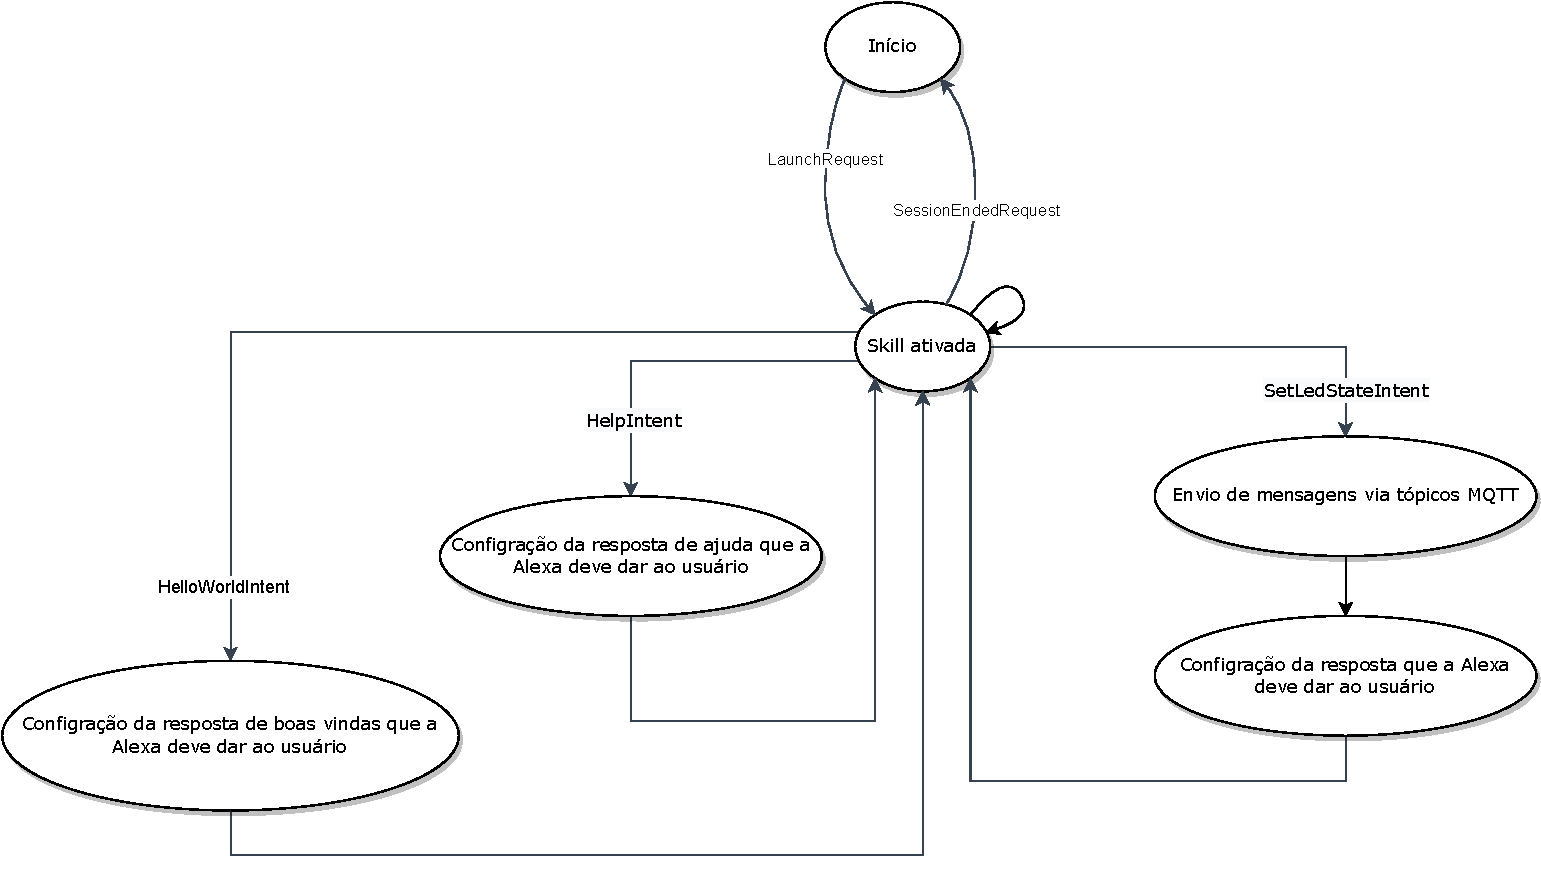
\includegraphics[scale=0.61]{Imagens/diagrama_de_estados_bl475eiot01a2_handler.pdf}
  \legend{Fonte: Produzido pelo autor (2022).}
  \label{fig:diagrama_de_estados_bl475eiot01a2_handler}
\end{figure}
